% Relatório da versão 1 do software ipump para o curso
% Sistemas de Controle - DCA0206 - UFRN
% Autores:
%   AUGUSTO MATHEUS PINHEIRO DAMASCENO
%   MARCEL DA CÂMARA RIBEIRO DANTAS
%   PABLO HOLANDA CARDOSO
%   PEDRO DE CASTRO GURGEL LIMA
%   RODRIGO DANTAS DA SILVA
% Modificado por: Ícaro Bezerra Queiroz de Araújo
%

%%%%%%%%%%%% STRUCTURE %%%%%%%%%%%%%%%
\documentclass[a4paper,12pt]{article}
\usepackage[T1]{fontenc}
\usepackage[utf8]{inputenc}
\usepackage[brazil]{babel}
\usepackage{lmodern}
\usepackage{setspace}
\usepackage[top=2cm, bottom=2cm, left=2cm, right=2cm]{geometry}
%%%%%%%%%%%%%%%%%%%%%%%%%%%%%%%%%%%%%%

%%%%%%%%%%%%%%%% PAGES STYLE %%%%%%%%%
\usepackage{fancyhdr}
\fancypagestyle{main}{
\renewcommand{\headrulewidth}{0pt}
\fancyhead[RO]{\thepage}
\fancyfoot[CO]{}
}
%%%%%%%%%%%%%%%%%%%%%%%%%%%%%%%%%%%%%%

\usepackage{graphicx}
\usepackage{float}
\usepackage{epstopdf}
\usepackage{subfig}
\usepackage{mathptmx}
\usepackage{changepage}


\usepackage{listings}
\usepackage{xcolor}
\lstset{language=C++,
                basicstyle=\ttfamily,
                keywordstyle=\color{blue}\ttfamily,
                stringstyle=\color{red}\ttfamily,
                commentstyle=\color{green}\ttfamily,
                morecomment=[l][\color{magenta}]{\#}
}

%\usepackage[alf]{abntex2cite}

%%%%%%%%%%% PDF METADATA %%%%%%%%%%%%%
\usepackage[ pdftitle={MODELO RELATÓRIO},
pdfsubject={INTRODUÇÃO AO LABORATÓRIO DE CONTROLE - Grupo 3},
pdfkeywords={Controle,Automação,UFRN,DCA,ipump},
hidelinks]{hyperref}
%%%%%%%%%%%%%%%%%%%%%%%%%%%%%%%%%%%%%%

\begin{document}

\onehalfspacing

\thispagestyle{empty}

\setcounter{page}{1}

%%%%%%%%%%%% LOGOS %%%%%%%%%%%%%%%%%%%

\begin{figure}[!ht]

\centering

\subfloat{

\includegraphics[width=2.7cm]{UFRN.eps}
\label{UFRN Logo}
}
\hspace{11.09cm}
\subfloat{

\includegraphics[width=2.4cm]{DCA.eps}
\label{DCA Logo}
}

%\caption{}
\label{Logos}

\end{figure}

%%%%%%%%%%%%%%% CAPA %%%%%%%%%%%%%%%%%

\vspace{-1cm}

\begin{center}
{\bf{\normalsize UNIVERSIDADE FEDERAL DO RIO GRANDE DO NORTE\\
CENTRO DE TECNOLOGIA\\
DEPARTAMENTO DE ENGENHARIA DE COMPUTAÇÃO E AUTOMAÇÃO\\
CURSO DE ENGENHARIA DE COMPUTAÇÃO
}}


\vspace{3.6cm}

{\bf{\large RELATÓRIO DA 3ª EXPERIÊNCIA\\
CONTROLE DE SISTEMAS DINÂMICOS: SISTEMA DE SEGUNDA ORDEM\\
}}
\vspace{1.5cm}
{\large TURMA: 01 A\\
	GRUPO Nº}

\vspace{3.6cm}


\begin{flushright}
\begin{normalsize}
ANDRESSA STÉFANY SILVA DE OLIVEIRA: 20160154101\\
\vspace{0.8cm}
FERNANDA MONTEIRO DE ALMEIDA: 20160154228\\
\vspace{0.8cm}
VITOR RAMOS GOMES DA SILVA: 20160154415\\
\vspace{0.8cm}
MÁRCIO LUIZ BEZERRA LOPES JÚNIOR: 20160154326\\
\end{normalsize}
\end{flushright}


\vspace{2.5cm}

{\large Natal-RN\\
2017}

\end{center}

\newpage

%%%%%%%%%%%%%%%  CONTRA-CAPA %%%%%%%%%

\thispagestyle{empty}

\begin{center}
\begin{normalsize}
ANDRESSA STÉFANY SILVA DE OLIVEIRA: 2016015410\\
\vspace{0.8cm}
FERNANDA MONTEIRO DE ALMEIDA 20160154228\\
\vspace{0.8cm}
VITOR RAMOS GOMES DA SILVA: 20160154415\\
\vspace{0.8cm}
MÁRCIO LUIZ BEZERRA LOPES JÚNIOR: 20160154326\\

\end{normalsize}
\end{center}
\vspace{3cm}

{\bf{\large {\centering CONTROLE DE SISTEMAS DINÂMICOS: SISTEMA DE SEGUNDA ORDEM\\}}}

\vspace{4cm}

\begin{adjustwidth}{7.5cm}{0cm}

{\normalsize

Terceiro Relatório apresentado à disciplina de
Laboratório de Sistemas de Controle, correspondente à
avaliação da 1º unidade do semestre 2017.1 do 8º período
do curso de Engenharia de Computação da
Universidade Federal do Rio Grande do Norte, sob
orientação do {\bf Prof. Fábio Meneghetti Ugulino de
Araújo.}

}

\end{adjustwidth}

\vspace{2cm}

\begin{center}

Professor:  Fábio Meneghetti Ugulino de Araújo.

\vspace{2.5cm}

{\large Natal-RN\\
2017}

\end{center}

\newpage

%%%%%%%%%%%%%%%  RESUMO %%%%%%%%%%%%%%

\thispagestyle{empty}

\begin{center}
{\large \textbf{RESUMO}}
\end{center}

\vspace{3cm}

\begin{flushleft}

\hspace{4ex}O presente trabalho é a terceira etapa da construção de um microcontrolador para controle de sistemas. Consiste no desenvolvimento de um software que se comunica com um sistema de tanques, uma planta Quanser, e seu simulador, com canais para leitura e escrita de sinais. Nesta etapa do trabalho, o objetivo foi a implementação de controladores P, PI, PD, PID e PI-D de segunda ordem. Também foram adicionados ao controlador quatro medidas para análise do sistema de tanques: tempos de subida, pico e acomodação, além do sobre-sinal máximo do sistema. As equações teóricas utilizadas para formular o controlador estão explicitadas no texto deste relatório, bem como os algoritmos que simulam seus funcionamentos. O comportamento do sistema pode ser observado pelo usuário através de três gráficos presentes na interface do software, um para o sinal de entrada e os demais para os canais de saída.\\

\end{flushleft}

\vspace{1.5cm}

\textbf{Palavras-chave:} sistema de tanques; sistema de controle; software; planta Quanser, controlador PID.

\newpage

%%%%%%%%% LISTA DE FIGURAS %%%%%%%%%%%

\thispagestyle{empty}

\begin{center}
\listoffigures
\end{center}

\newpage

%%%%%%%%%%%%%%% SUMÁRIO %%%%%%%%%%%%%%

\thispagestyle{empty}

\begin{center}
\tableofcontents
\end{center}

\newpage

%%%%%%%%%%%%%%% INTRODUÇÃO %%%%%%%%%%%

\thispagestyle{main}

\section{INTRODUÇÃO}

\begin{flushleft}
\hspace{4ex}A prática de laboratório 04 tem como objetivo introduzir um sistema de controle em cascata na planta \textit{Quanser}, sendo a figura \ref{r2d2e} o simulador da planta:

\begin{figure}[H]
\centering
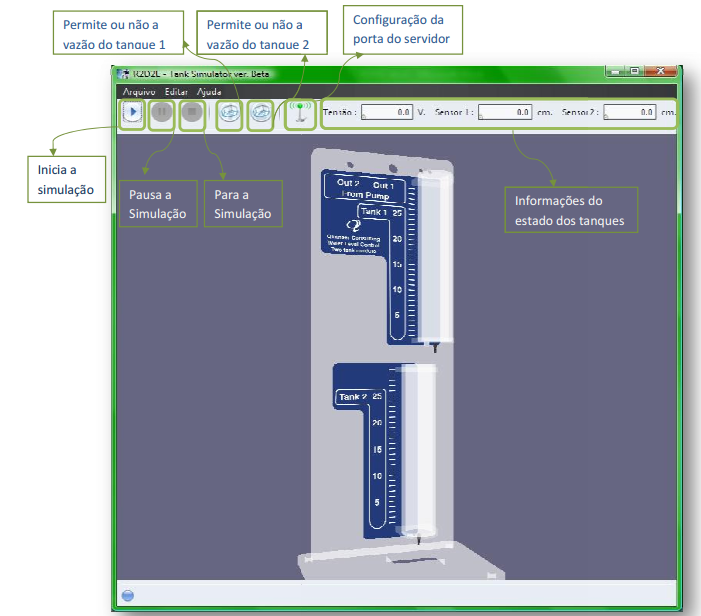
\includegraphics[width=11cm]{ImagensLab4/simulator.png}
\caption{R2D2E - Tank Simulator}
\label{r2d2e}
\end{figure}

\hspace{4ex}Pretende-se controlar o nível de água de ambos os tanques da planta, para isso, foi implementado os controladores Proporcional (P), Proporcional Integrativo (PI), Proporcional Derivativo (PD), Proporcional Integrativo Derivativo (PID) e Proporcional Integrativo Derivativo em controle de ação baseado no sinal do processo (PI-D). Quem irá escolher qual controle será usado é o usuário, através da interface do programa desenvolvido, como mostrado na figura \ref{interface}:

\begin{figure}[H]
\centering
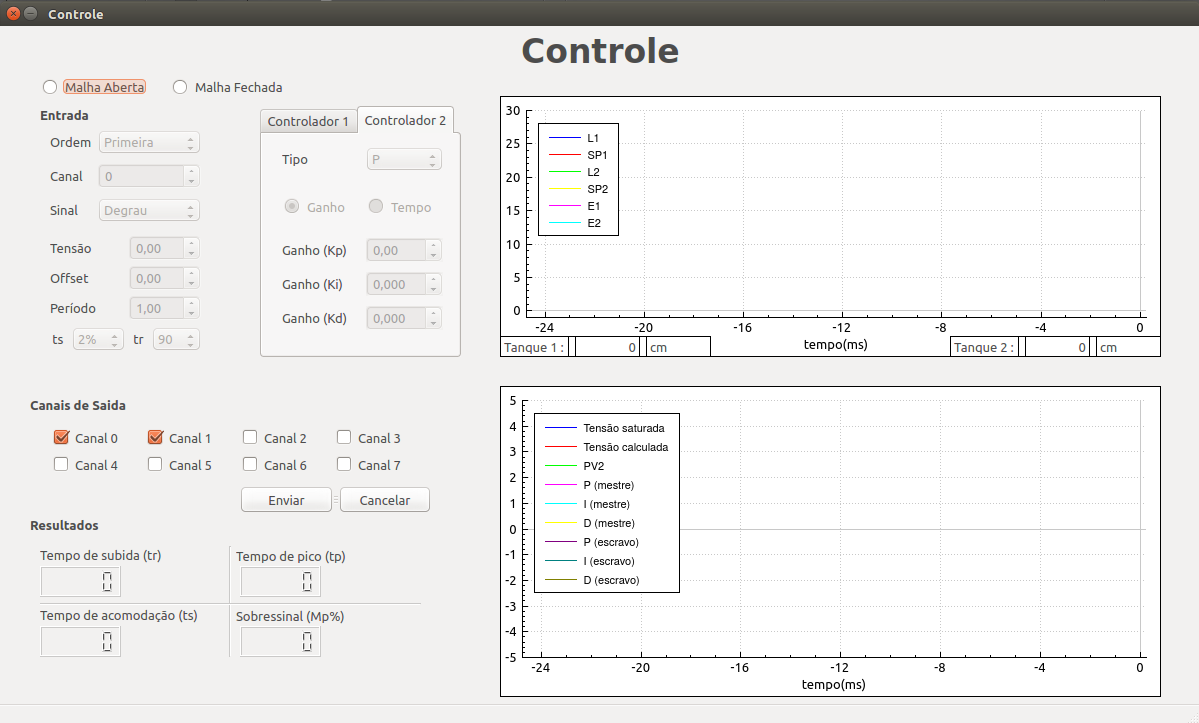
\includegraphics[width=11cm]{ImagensLab4/interface-versao4.png}
\caption{Interface do software de controle}
\label{interface}
\end{figure}

\hspace{4ex}Além dessas opções, o usuário também deve escolher os ganhos dos controladores Kp, Ki e ou Kd, ou $\tau_i$ e $\tau_d$, o  sinal de referência a ser enviado, o offset, a análise da resposta do sistema para o tempo de subida (t$_r$), por exemplo, de 5\% à 95\%, e o tempo de acomodação (t$_s$), para as faixas de 2\%, 5\% e 10\% do degrau. Ademais, é possível saber os valores do  t$_r$, t$_s$, tempo de pico (t$_p$) e o sobressinal (Mp) do sistema de segunda ordem.

\hspace{4ex}No relatório é apresentado como foi a metodologia, os resultados obtidos através de testes e as conclusões a partir da comparação do comportamento do sistema com uma e com duas malhas.

\end{flushleft}

\newpage

%%%%%%%%%% REFERENCIAL TEÓRICO %%%%%%%

\thispagestyle{main}

\section{REFERENCIAL TEÓRICO}

\hspace{4ex}O sistema de controle da planta mostrada na figura \ref{quaser} é caracterizado como sistema de segunda ordem quando se pretende controlar o nível do tanque de baixo, pois sua alimentação é a vazão do tanque de cima.

\begin{figure}[h]
\centering
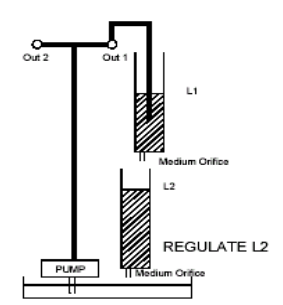
\includegraphics[width=5cm]{fotosLab3/planta.png}
\caption{Planta Quaser}
\label{quaser}
\end{figure}

\hspace{4ex}Tendo o objetivo de comparar controladores, utiliza-se algumas medidas de desempenho, como, o tempo de subida, o tempo de acomodação, o tempo de pico e o overshoot.

\hspace{4ex}O tempo de subida(t$_r$) é o tempo em que a variável manipulada sai da referência atual e chega na nova referência. Para um sistema de segunda ordem ideal:

\begin{center}
$ t_r = \frac{\pi - \beta}{w_d} $
\end{center} 

\hspace{4ex}O tempo de acomodação é o tempo em que é a variável manipulada levou para entrar em uma região de acomodação e não sair mais.

\begin{center}
$ t_s=\frac{3}{\xi w_n} $
\end{center}

\hspace{4ex}O tempo de pico é o tempo em que o sinal levou para atingir o seu maior valor, e o overshoot é a porcentagem do erro com relação ao setpoint.

\begin{center}
$ t_p=\frac{\pi}{w_d} $\\
$ M_p(\%)=100( e^{- \frac{\xi\pi}{\sqrt{1-\xi^{2}}} } ) $
\end{center}

Na figura \ref{curva} pode ser visto a representação desses tempos mencionados acima.

\begin{figure}[H]
\centering
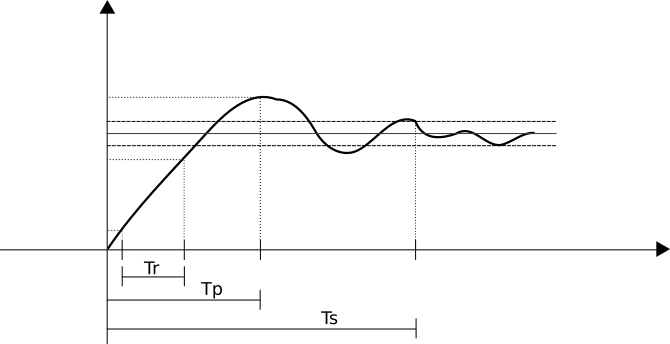
\includegraphics[width=15cm]{fotosLab3/ref.png}
\caption{Curva}
\label{curva}
\end{figure}


\hspace{4ex}Essas medidas também servem para analisar o que acontece quando mudamos os ganhos dos controladores, e elas nos ajudam a decidir qual o melhor controlador segundo as especificações de desempenho.


\newpage

%%%%%%%%%% METODOLOGIA %%%%%%%%%%%%%%%

\thispagestyle{main}

\section{METODOLOGIA}

\hspace{4ex}Utilizando o simulador R2D2E, foram feitos testes com o controlador mestre e o escravo, como também, com apenas um controlador para alcançar determinados níveis dos tanques da planta, os quais serão expostos nos resultados.

\hspace{4ex}Para isso, foi implementado uma classe controlador a qual é determinada de acordo com as escolhas do usuário, ou seja, se é P, PI, PD, PID ou PI-D. Por exemplo, se o usuário escolhe o controlador PD, ele fornecerá apenas os valores de Kp e Kd, ou Kp e $\tau_d$, e a partir desses valores a classe assumirá que Ki ou $\tau_i$ não existe, ou seja, o valor da integral será zero. O mesmo acontece se for escolhido o PI, nesse caso, o valor da derivada do erro será zero. Observe o método abaixo:
\\
\begin{lstlisting}
double PID::Controle(double e, double h)
//Metodo para os controladores P, PI, PD e PID
{
    I= I+Ki*e*h; //Simpsons (e+e_ant)*h/2 - integral do erro
    D= Kd*(e-e_ant)/h; //Derivada do erro
    e_ant= e; //Erro
    return Kp*e+I+D; //Sinal de controle
}

double PID::Controle(double e, double y, double h)
//Metodo para o controlador PI-D
{
    I= I+Ki*e*h;
    D= Kd*(y-e_ant)/h;
    e_ant= y;
    return Kp*e+I+D;
}
\end{lstlisting}

\hspace{4ex}No software desenvolvido, esses valores podem ser escolhidos como mostrado na figura \ref{controladores}.

\begin{figure}[H]
     \centering
     \subfloat[][Controlador Mestre]{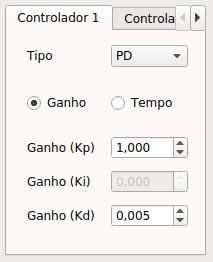
\includegraphics[width=4cm]{ImagensLab4/controlador1}\label{<figureP1>}}\hspace{4ex}
     \subfloat[][Controlador Escravo]{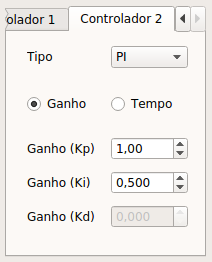
\includegraphics[width=4cm]{ImagensLab4/controlador2}\label{<figureP2>}}\\
     \caption{Interface para a escolha dos controladores}
     \label{fig:controladores}
\end{figure}


\newpage

%%%%%%%%%% RESULTADOS %%%%%%%%%%%%%%%

\thispagestyle{main}

\section{RESULTADOS}

\hspace{4ex}A análise feita teve como foco a análise do desempenho do sistema de segunda ordem através de tempos específicos. Ou seja, o objetivo era controlar o segundo tanque do sistema, as leituras do nível aparecem no gráfico localizado inferior da janela.

\hspace{4ex}O primeiro teste foi feito utilizando o controle PI, na figura \ref{<figureP1>} se pode perceber o efeito do sobressinal negativo, onde se alcançou cerca de quase 18\% de  abaixo do nível estabelecido. Essa porcentagem é em relação a diferença do nível anterior para o nível configurado atualmente. No caso, alterou-se de 20 cm para 10 cm.

\hspace{4ex}Na figura \ref{<figureP2>}, nota-se claramente o tempo de subida de 12,3 s. Alguns valores como sobressinal e tempo de acomodação são atualizados constamente e mostrados durante o cálculo, então o valor real só extraído quando o sistema entra em regime permanente.
\begin{figure}[H]
     \centering
     \subfloat[][]{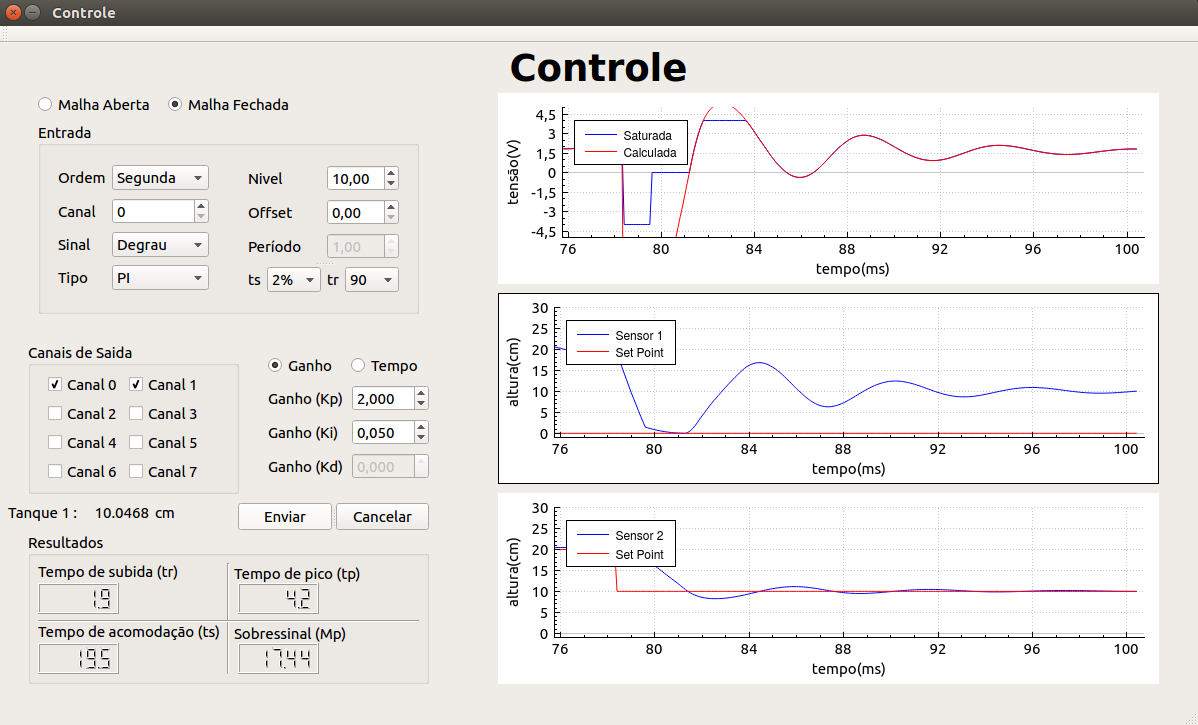
\includegraphics[width=10cm]{resultados-lab3/03}\label{<figureP1>}}\hspace{4ex}
     \subfloat[][]{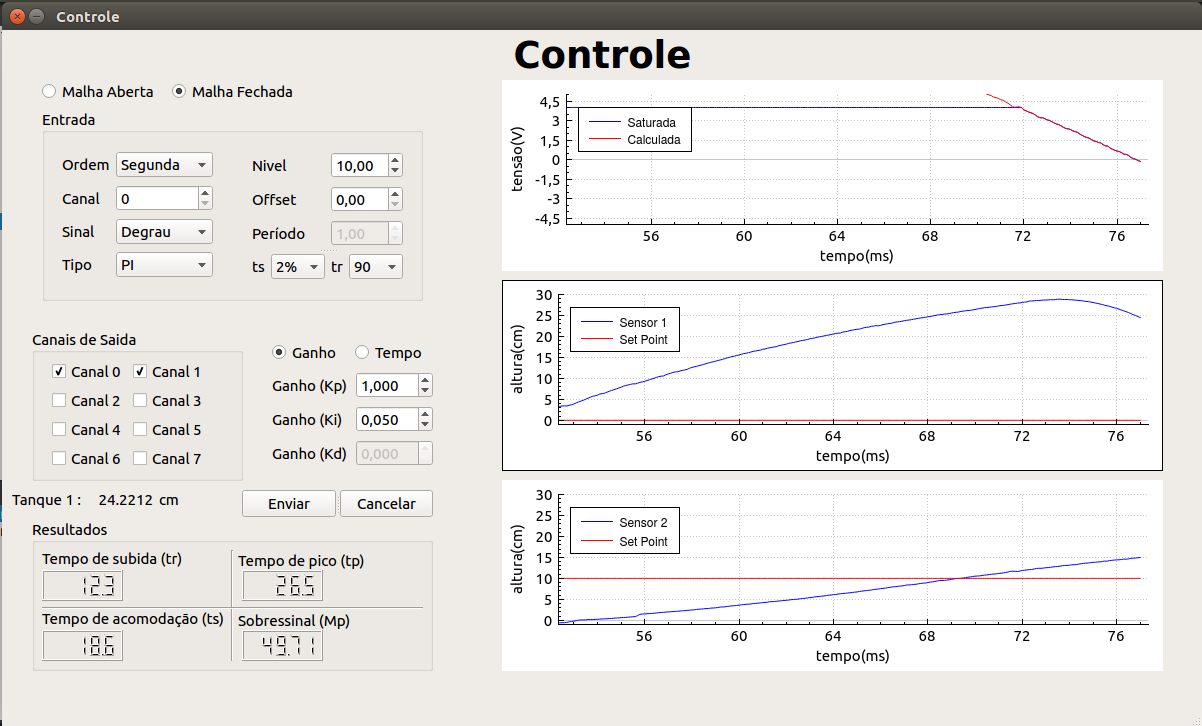
\includegraphics[width=10cm]{resultados-lab3/04}\label{<figureP2>}}\\
     
     \caption{Análise do Controle PI}
     \label{fig:ControlePI}
\end{figure}

\hspace{4ex}Já no primeiro teste, notou-se que o controle do segundo tanque levou mais tempo para responder aos níveis de referência.

\hspace{4ex}Na \ref{<figurePID1>}, vê-se novamente o sobressinal agora positivo. O tempo de pico é calculado junto com o sobressinal e é mostrado logo acima do $M_p$ na parte de resultados do programa.

\hspace{4ex}Nas figuras \ref{<figurePID2>} e \ref{<figurePID3>}, mostra-se o tempo de acomodação obtido, 35 s. Foi considerado uma faixa de tolerância de 2\% que pode ser alterada pelo usuário. Percebe-se que os valores obtidos são uma boa aproximação, já que não se pode obter um tempo mais preciso devido à taxa de leitura dos sensores e resposta do sistema.
\begin{figure}[H]
     \centering
     \subfloat[][]{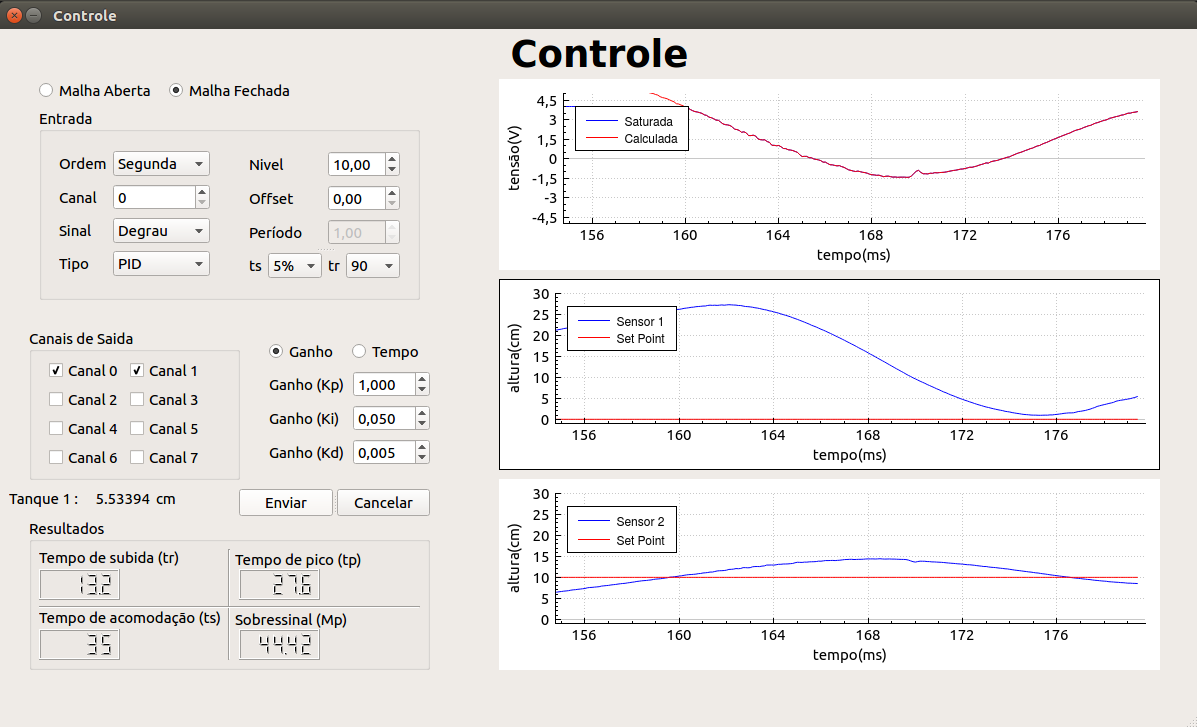
\includegraphics[width=10cm]{resultados-lab3/05}\label{<figurePID1>}}\hspace{4ex}
     \subfloat[][]{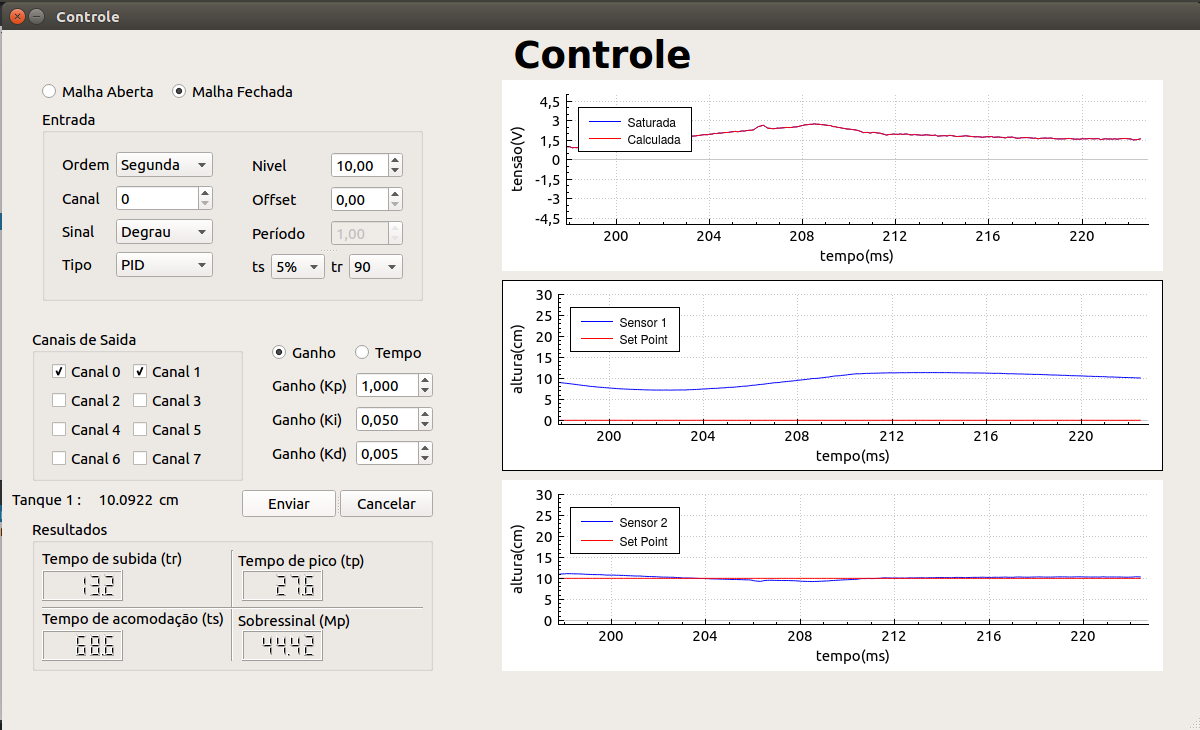
\includegraphics[width=10cm]{resultados-lab3/06}\label{<figurePID2>}}\\
     \subfloat[][]{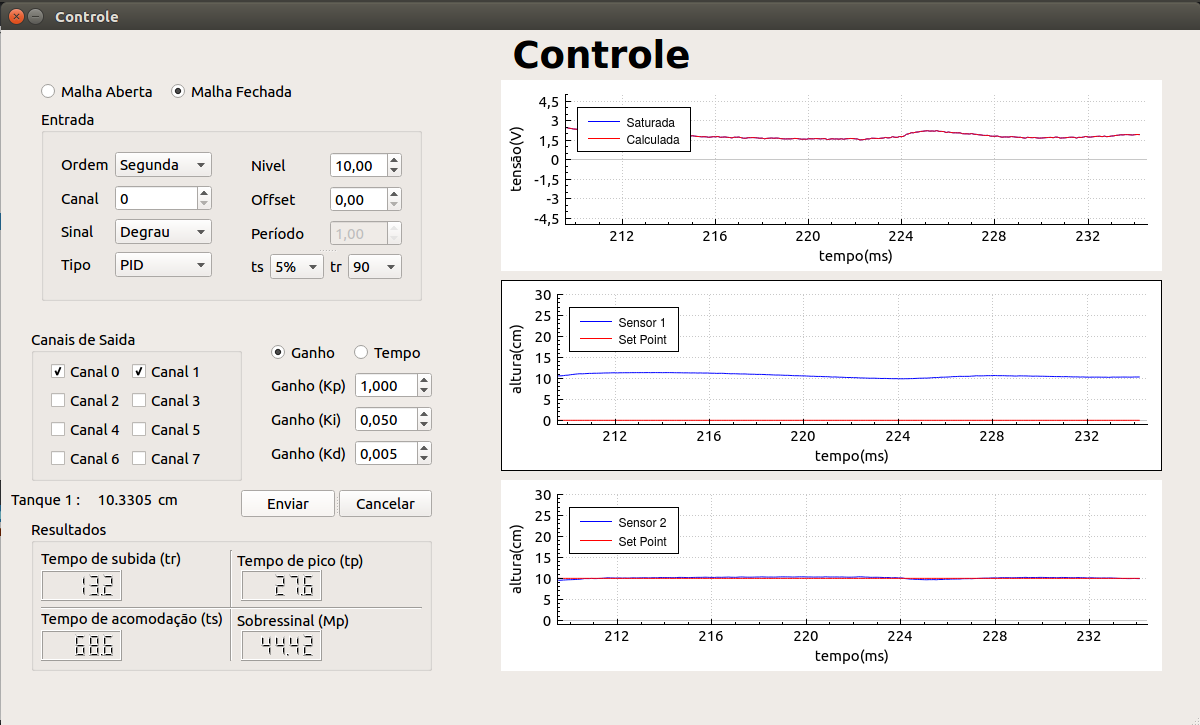
\includegraphics[width=10cm]{resultados-lab3/07}\label{<figurePID3>}}
     
     \caption{Análise do Controle PID}
     \label{controlePID}
\end{figure}

\hspace{4ex} O efeito dos controladores no sistema continua o mesmo encontrado no sistema de primeira ordem. A oscilação do efeito derivativo e a resposta mais agressiva do efeito da integração. Sendo que como o sistema tem uma resposta mais lenta, faz-se necessário a análise dos tempos de subida, sobressinal e tempo de acomodação para os devidos ajustes nas constantes $K_p$, $K_D$ e $K_I$. Por exemplo, se o tempo de subida foi muito longo, é necessário o aumento do $K_I$ para uma resposta mais rápida. Mas devido aos efeitos de wind up do integrador e a amplificação do ruído no derivativo, o controlador precisa de filtros. No programa não foi implementado esse filtros, o que limita as faixas de uso das constantes. 


\begin{figure}[H]
     \centering
     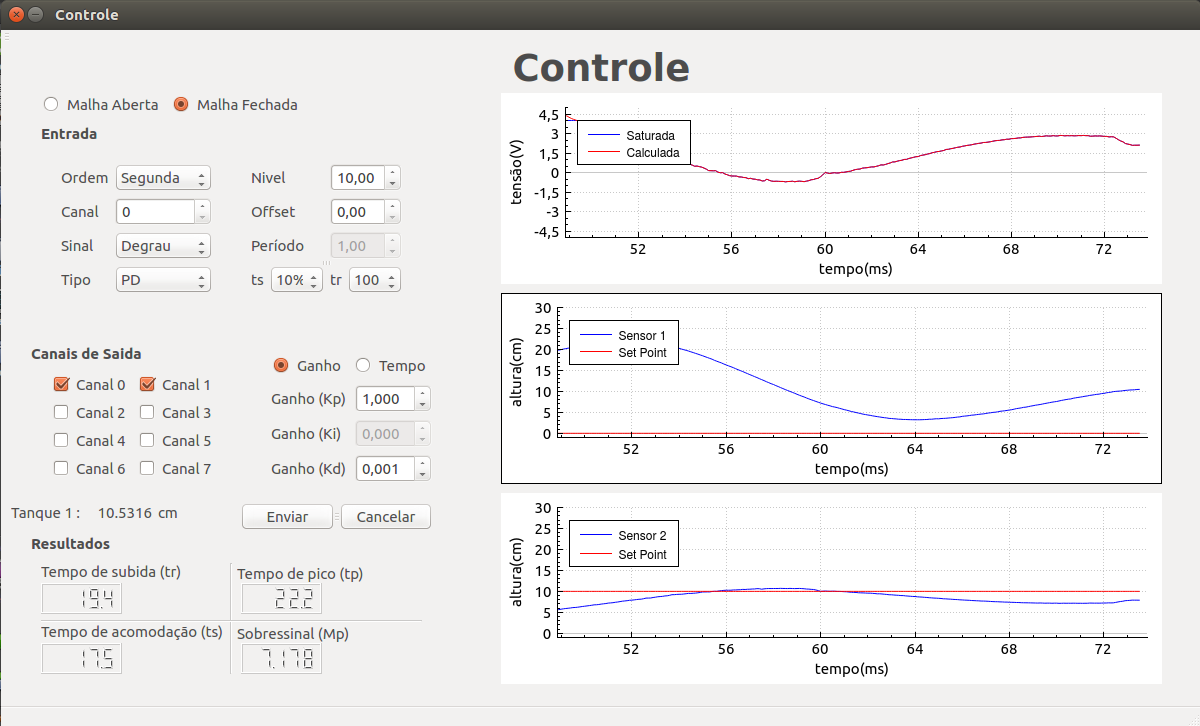
\includegraphics[width=10cm]{resultados-lab3/19}\label{<figurePD1>}
     \caption{Análise do Controle PD}
     \label{controlePD}
\end{figure}

Por fim o teste feito com o controlador PD. Foi usado uma constante $K_D$ baixa para evitar os efeitos negativos.



\newpage

%%%%%%%%%% CONCLUSÃO %%%%%%%%%%%%%%%

\thispagestyle{main}

\section{CONCLUSÃO}


\hspace{4ex}Os testes realizados num sistema de segunda ordem mostraram a importância da análise dos tempo de subida, tempo de pico, sobressinal e tempo de acomodação para o controle de um sistema. Estes valores obtidos experimentalmente podem ser aplicados no modelo matemático, para então encontrar a função que rege o sistema podendo assim ser mais fácil sintonizar o controlador e projetar. Como foi utilizado teorias aplicadas para sistemas lineares, essas soluções podem ser generalizadas e adaptadas para qualquer sistema linear. 
\newpage

%%%%%%%% REFERÊNCIAS %%%%%%%%%%%%%%%%%

%\thispagestyle{empty}
%\section{BIBLIOGRAFIA}
 %.
 
%Dorf, R.; Bishop, R. Sistemas de controle modernos. Rio de Janeiro (RJ): LTC, 2009. 

%Ogata, K. Modern control engineering. Boston: Prentice Hall, 2010.


%Referências bibliogáficas (geradas automaticamente)
%\addcontentsline{toc}{chapter}{Referências bibliográficas}
%\bibliography{bib/bibliografia}

%Apêndice A
%\include{apendice}

\end{document}
